\section{Local Polynomial Regression}

  Now another way to think about the kernel estimator is as such. Suppose that you're doing linear regression on a bunch of points and you want to choose a $c$ that minimizes the loss. 
  \begin{equation}
    \sum_i (Y_i - c)^2
  \end{equation}
  You would just pick $c = \hat{Y}$. But if you are given some sort of locality condition, that the value of $c$ should depend more on the values closer to it, you're really now minimizing 
  \begin{equation}
    \sum_i (Y_i - c(x))^2 K \bigg( \frac{X_i - x}{h} \bigg)
  \end{equation}
  Minimizing this by setting the derivative equal to $0$ and solving gives us the kernel estimator. Therefore you're fitting some sort of local constant at a point $X$. But why fit a local constant, when you can fit a local line or polynomial? This is the idea behind local polynomial regression.

  \begin{figure}[H]
    \centering 
    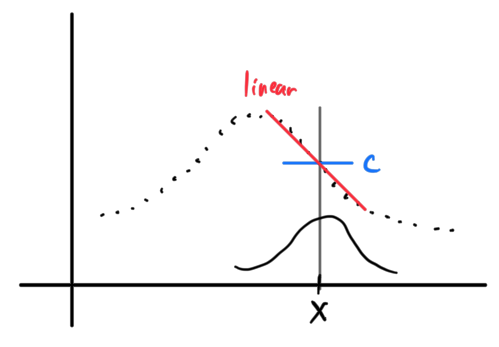
\includegraphics[scale=0.4]{img/local_linear_estimator.png}
    \caption{Rather than using a local constant, we can use a local linear estimator.} 
    \label{fig:local_linear_estimator}
  \end{figure}

  Therefore, we can minimize the modified loss. 

  \begin{definition}[Local Polynomial Estimator]
    The \textbf{local polynomial estimator} is a local linear kernel smoother that estimates the function $\hat{f}$ that minimizes the following loss. 
    \begin{equation}
      \argmin_{\beta} \sum_i K \bigg( \frac{X_i - x}{h} \bigg) \big( Y_i - (\beta_0 (x) - \beta_1 (x) (x- X_i) + \ldots + \beta_k (x) (x - X_i)^k )\big)
    \end{equation}
  \end{definition}

  So we can fit a line 
  \begin{equation}
    f(\mu) \approx \hat{\beta}_0 (x) + \hat{\beta}_1 (x) (\mu - x)
  \end{equation}
  and simply remove the intercept term to get the local linear estimator. 
  \begin{equation}
    \hat{f}(x) = \hat{\beta}_0 (x)
  \end{equation}
  Note that this is not the same as taking the constant estimate. We are extracting the fitted intercept term and so $\hat{\beta}_0(x) \neq c(x)$. 

  \begin{theorem}[Weighted Least Squares]
    The solution to the local linear estimator is similar to the weighted least squares solution. 
    \begin{equation}
      \hat{\beta}(x) = \begin{pmatrix} \hat{\beta}_0 (x) \\ \hat{\beta}_1 (x) \end{pmatrix} = (X^T W X)^{-1} X^T W Y
    \end{equation}
    where 
    \begin{equation}
      X = \begin{pmatrix} 1 & X_1 - x \\ \vdots & \vdots \\ 1 & X_n - x \end{pmatrix} \qquad W = \begin{pmatrix} K \bigg( \frac{X_1 - x}{h} \bigg) & 0 & \cdots & 0 \\ 0 & K \bigg( \frac{X_2 - x}{h} \bigg) & \cdots & 0 \\ \vdots & \vdots & \ddots & \vdots \\ 0 & 0 & \cdots & K \bigg( \frac{X_n - x}{h} \bigg) \end{pmatrix}
    \end{equation}
  \end{theorem}

  Computationally, it's similar to kernel regression and it gets rid of both the boundary and design bias. 

